\documentclass[aspectratio=169,11pt]{beamer}


\usepackage[utf8]{inputenc}
\usepackage[T1]{fontenc}
\usepackage[brazil]{babel}
\usepackage{lmodern}

\usepackage{graphicx}
\usepackage{tikz}
\usepackage{xcolor}
\usepackage{ragged2e}
\usepackage{booktabs}
\usepackage{array}
\usepackage{amsmath}
\usepackage{hyperref}

\usetikzlibrary{
    positioning,
    calc,
    shapes.geometric,
    arrows.meta
}


\usepackage[
    backend=biber,
    style=authoryear,
    maxcitenames=2,
    maxbibnames=99,
    giveninits=true
]{biblatex}

\addbibresource{referencias.bib}


\definecolor{AzulEscuro}{HTML}{183642}
\definecolor{AzulMedio}{HTML}{28666E}
\definecolor{AzulClaro}{HTML}{DCECEF}

\definecolor{Papel}{HTML}{F4EBDD}
\definecolor{Sepia}{HTML}{8B6846}
\definecolor{MarromEscuro}{HTML}{49382B}

\definecolor{CinzaTexto}{HTML}{30363A}
\definecolor{CinzaClaro}{HTML}{E9ECEF}
\definecolor{CinzaMedio}{HTML}{889297}
\definecolor{Branco}{HTML}{FFFFFF}

\definecolor{Destaque}{HTML}{C65D3B}


\setbeamertemplate{navigation symbols}{}

\setbeamercolor{normal text}{
    fg=CinzaTexto,
    bg=Branco
}

\setbeamercolor{frametitle}{
    fg=AzulEscuro,
    bg=Branco
}

\setbeamercolor{structure}{
    fg=AzulMedio
}

\setbeamercolor{alerted text}{
    fg=Destaque
}

\setbeamerfont{frametitle}{
    size=\Large,
    series=\bfseries
}

\setbeamerfont{title}{
    size=\LARGE,
    series=\bfseries
}

\setbeamerfont{subtitle}{
    size=\large
}

\setbeamersize{
    text margin left=0.75cm,
    text margin right=0.75cm
}


\setbeamertemplate{footline}{
    \leavevmode
    \hbox{
        \begin{beamercolorbox}[
            wd=.80\paperwidth,
            ht=2.7ex,
            dp=1.2ex,
            leftskip=.7cm
        ]{author in head/foot}
            \color{CinzaMedio}
            \scriptsize Visualização de dados
        \end{beamercolorbox}

        \begin{beamercolorbox}[
            wd=.20\paperwidth,
            ht=2.7ex,
            dp=1.2ex,
            rightskip=.7cm
        ]{date in head/foot}
            \hfill
            \color{CinzaMedio}
            \scriptsize
            \insertframenumber/\inserttotalframenumber
        \end{beamercolorbox}
    }
}


\addtobeamertemplate{frametitle}{}{
    \vspace{-0.2cm}

    \begin{tikzpicture}
        \draw[
            AzulMedio,
            line width=0.7pt
        ]
        (0,0) -- (\textwidth,0);
    \end{tikzpicture}

    \vspace{-0.2cm}
}

\newcommand{\etiqueta}[1]{
    \tikz[baseline]
    \node[
        fill=AzulClaro,
        text=AzulEscuro,
        rounded corners=2pt,
        inner xsep=6pt,
        inner ysep=3pt,
        font=\scriptsize\bfseries
    ]{#1};
}


\begin{document}


{
\setbeamertemplate{footline}{}

\begin{frame}[plain]

    \begin{tikzpicture}[remember picture,overlay]

        \fill[Papel]
        (current page.north west)
        rectangle
        ($(current page.south west)+(0.37\paperwidth,0)$);

        \fill[AzulEscuro]
        ($(current page.north east)+(-0.035\paperwidth,0)$)
        rectangle
        (current page.south east);

        \draw[
            Sepia,
            opacity=.5,
            line width=.8pt
        ]
        ($(current page.north west)+(0.37\paperwidth,-0.7cm)$)
        --
        ($(current page.south west)+(0.37\paperwidth,0.7cm)$);

        \draw[
            Sepia,
            opacity=.18,
            line width=1.2pt
        ]
        ($(current page.center)+(-5.2cm,-1.8cm)$)
        circle (1.45cm);

        \draw[
            Sepia,
            opacity=.18
        ]
        ($(current page.center)+(-6.65cm,-1.8cm)$)
        --
        ($(current page.center)+(-3.75cm,-1.8cm)$);

        \draw[
            Sepia,
            opacity=.18
        ]
        ($(current page.center)+(-5.2cm,-3.25cm)$)
        --
        ($(current page.center)+(-5.2cm,-0.35cm)$);

    \end{tikzpicture}

    \vspace{1.25cm}

    \hspace{0.8cm}
    \begin{minipage}{0.78\textwidth}

        {\color{AzulMedio}
        \small
        HISTÓRIA + PERCEPÇÃO + DESIGN}

        \vspace{0.4cm}

        {\color{AzulEscuro}
        \fontsize{27}{31}\selectfont
        \bfseries
        Redesenhando\\
        gráficos históricos}

        \vspace{0.45cm}

        {\color{CinzaTexto}
        \large
        O que os princípios modernos de visualização
        podem acrescentar às primeiras representações
        de dados?}

        \vspace{0.8cm}

        {\small
        textbf{Heitor Fernandes, Kaue Badia \& Julio Freitas}
        \hspace{0.2cm}
        {\color{CinzaMedio}$\vert$}
        \hspace{0.2cm}
        Visualização de Dados}

    \end{minipage}

\end{frame}

}


\begin{frame}{A pergunta}

    \vspace{0.15cm}

    \begin{columns}[T,onlytextwidth]


        \begin{column}{0.37\textwidth}

            \centering

            \begin{tikzpicture}

                \node[
                    fill=Papel,
                    rounded corners=4pt,
                    minimum height=5.2cm,
                    text width=0.82\linewidth,
                    inner sep=8pt,
                    align=center
                ]{
                    {\color{Sepia}\Large\textbf{1644}}\\[0.25cm]
                    {\color{MarromEscuro}\textbf{Van Langren}}\\[0.45cm]
                    {\color{MarromEscuro}
                    Uma das primeiras\\
                    visualizações estatísticas}\\[0.45cm]
                    {\color{Sepia}\Large$\downarrow$}\\[0.45cm]
                    {\color{MarromEscuro}
                    \textbf{Como representaríamos\\
                    esses dados hoje?}}
                };

            \end{tikzpicture}

        \end{column}


        \begin{column}{0.10\textwidth}

            \centering
            \vspace{2.0cm}

            {\color{Destaque}
            \Large
            $\longrightarrow$}

        \end{column}


        \begin{column}{0.49\textwidth}

            \vspace{0.8cm}

            \begin{center}
            {\color{AzulEscuro}
            \Large
            \textbf{Pergunta central} }
            

            \vspace{0.45cm}

            \begin{tikzpicture}

                \node[
                    draw=AzulMedio,
                    line width=1pt,
                    rounded corners=4pt,
                    inner sep=8pt,
                    text width=0.82\linewidth,
                    align=left
                ]{
                    \textit{
                    Como visualizações históricas podem ser
                    redesenhadas utilizando princípios modernos
                    de visualização de dados?
                    }
                };

            \end{tikzpicture}
            \end{center}

        \end{column}

    \end{columns}

\end{frame}


\begin{frame}{Como avaliar uma visualização?}

    \vspace{0.35cm}

    \begin{columns}[T,onlytextwidth]


        \begin{column}{0.22\textwidth}
            \centering

            \begin{tikzpicture}
                \node[
                    fill=AzulClaro,
                    rounded corners=5pt,
                    minimum height=3.35cm,
                    text width=0.82\linewidth,
                    inner sep=6pt,
                    align=center
                ]{
                    {\color{AzulEscuro}
                    \fontsize{22}{22}\selectfont
                    $\bullet$}\\[0.30cm]
                    {\bfseries Dados}\\[0.30cm]
                    {\scriptsize
                    O que precisa\\
                    aparecer?}
                };
            \end{tikzpicture}

        \end{column}


        \begin{column}{0.22\textwidth}
            \centering

            \begin{tikzpicture}
                \node[
                    fill=Papel,
                    rounded corners=5pt,
                    minimum height=3.35cm,
                    text width=0.82\linewidth,
                    inner sep=6pt,
                    align=center
                ]{
                    {\color{Sepia}
                    \fontsize{22}{22}\selectfont
                    $\blacktriangle$}\\[0.30cm]
                    {\bfseries Hierarquia}\\[0.30cm]
                    {\scriptsize
                    Para onde o olhar\\
                    vai primeiro?}
                };
            \end{tikzpicture}

        \end{column}


        \begin{column}{0.22\textwidth}
            \centering

            \begin{tikzpicture}
                \node[
                    fill=CinzaClaro,
                    rounded corners=5pt,
                    minimum height=3.35cm,
                    text width=0.82\linewidth,
                    inner sep=6pt,
                    align=center
                ]{
                    {\color{CinzaTexto}
                    \fontsize{22}{22}\selectfont
                    $\leftrightarrow$}\\[0.30cm]
                    {\bfseries Comparação}\\[0.30cm]
                    {\scriptsize
                    É fácil comparar\\
                    os valores?}
                };
            \end{tikzpicture}

        \end{column}


        \begin{column}{0.22\textwidth}
            \centering

            \begin{tikzpicture}
                \node[
                    fill=AzulEscuro,
                    text=white,
                    rounded corners=5pt,
                    minimum height=3.35cm,
                    text width=0.82\linewidth,
                    inner sep=6pt,
                    align=center
                ]{
                    {\color{white}
                    \fontsize{22}{22}\selectfont
                    $\times$}\\[0.30cm]
                    {\bfseries Ruído}\\[0.30cm]
                    {\scriptsize
                    O que pode ser\\
                    retirado?}
                };
            \end{tikzpicture}

        \end{column}

    \end{columns}

    \vspace{0.55cm}

    \begin{center}
        {\small
        \color{CinzaMedio}
        Gestalt \parencite{wagemans2012}
        \quad $\cdot$ \quad
        percepção visual \parencite{cairo2012}
        \quad $\cdot$ \quad
        elementos visuais
        \quad $\cdot$ \quad
        princípios de Tufte \parencite{tufte2001}}
    \end{center}

\end{frame}


\begin{frame}{Exemplo 1 — Van Langren, 1644}

    \vspace{0.05cm}

    \begin{columns}[T,onlytextwidth]


        \begin{column}{0.56\textwidth}

            \etiqueta{ORIGINAL}

            \vspace{0.22cm}

            \centering

            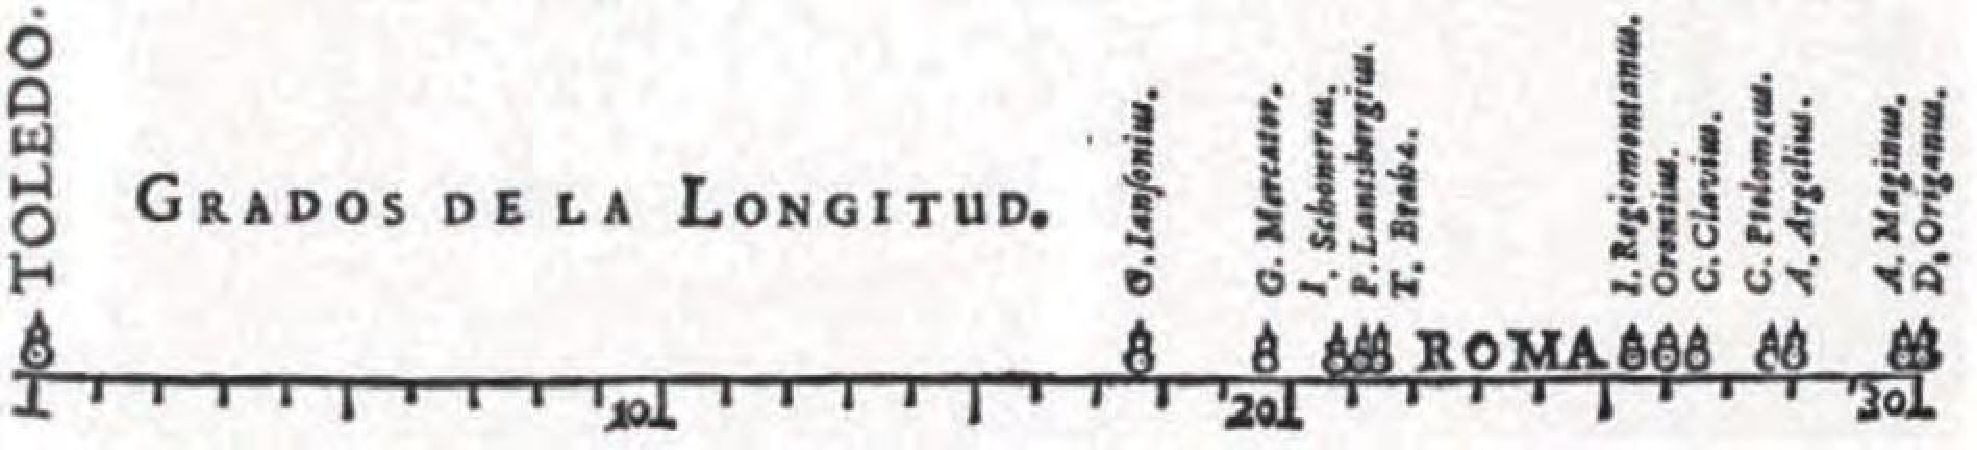
\includegraphics[
                width=0.97\linewidth,
                keepaspectratio
            ]{imagens/van_langren_original.pdf}

            \vspace{0.12cm}

            {\scriptsize
            \color{CinzaMedio}
            Fonte: \textcite{tufte1997};
            reproduzido em \textcite{ara2025}.}


            \vspace{0.42cm}

            \begin{tikzpicture}
                \node[
                    fill=AzulClaro,
                    rounded corners=4pt,
                    inner sep=8pt,
                    text width=0.90\linewidth,
                    align=left
                ]{
                    {\color{AzulEscuro}
                    \textbf{Como a leitura acontece?}}

                    \par\vspace{0.18cm}

                    {\small
                    A posição horizontal representa a estimativa.
                    A distância entre as marcas torna imediatamente
                    visível a divergência entre os valores.}
                };
            \end{tikzpicture}

        \end{column}


        \begin{column}{0.41\textwidth}

            \raggedright

            \etiqueta{LEITURA}

            \vspace{0.30cm}


            {\small
            \color{AzulEscuro}
            \textbf{O que está sendo mostrado?}}

            \vspace{0.12cm}

            {\footnotesize
            O gráfico mostra diferentes estimativas para a distância, em graus de longitude, entre Toledo e Roma. Cada estimativa é marcada pelo nome do astrônomo que a propôs.
            }

            \vspace{0.32cm}
            

            {\small
            \color{AzulEscuro}
            \textbf{O que poderia mudar?}}

            \vspace{0.12cm}

            {\footnotesize
            Rótulos mais legíveis, uma escala mais clara
            e maior destaque para cada observação.
            }

        \end{column}

    \end{columns}

\end{frame}

\begin{frame}{O mesmo dado, outra linguagem visual}

    \vspace{0.05cm}

    \begin{columns}[T,onlytextwidth]


        \begin{column}{0.4\textwidth}

            {\color{Sepia}
            \small
            \textbf{1644}}

            \vspace{0.15cm}

            \centering

            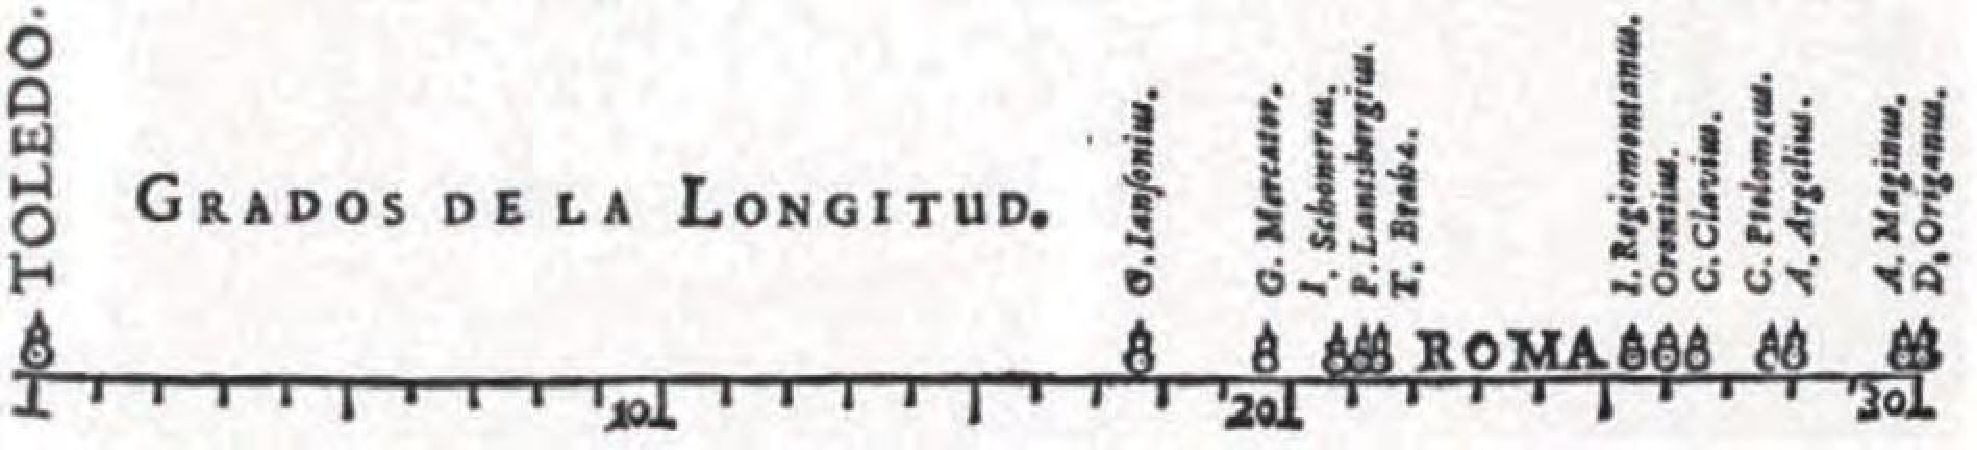
\includegraphics[
                width=\linewidth,
                height=0.37\textheight,
                keepaspectratio
            ]{imagens/van_langren_original.pdf}

            \vspace{0.10cm}

            {\scriptsize
            \color{CinzaMedio}
            Fonte: \textcite{tufte1997};
            reproduzido em \textcite{ara2025}.}

            \vspace{0.28cm}


            \begin{tikzpicture}
                \node[
                    fill=AzulClaro,
                    rounded corners=3pt,
                    inner sep=7pt,
                    text width=0.90\linewidth,
                    align=left
                ]{
                    \small
                    \textbf{Mudanças principais:}

                    \par\vspace{0.12cm}

                    Agora cada astrônomo ocupa a própria linha; as estimativas estão ordenadas por longitude; o valor real foi adicionado como referência.
                };
            \end{tikzpicture}

        \end{column}


        \begin{column}{0.59\textwidth}

            {\color{AzulMedio}
            \small
            \textbf{REDESENHO}}

            \vspace{0.15cm}

            \centering

            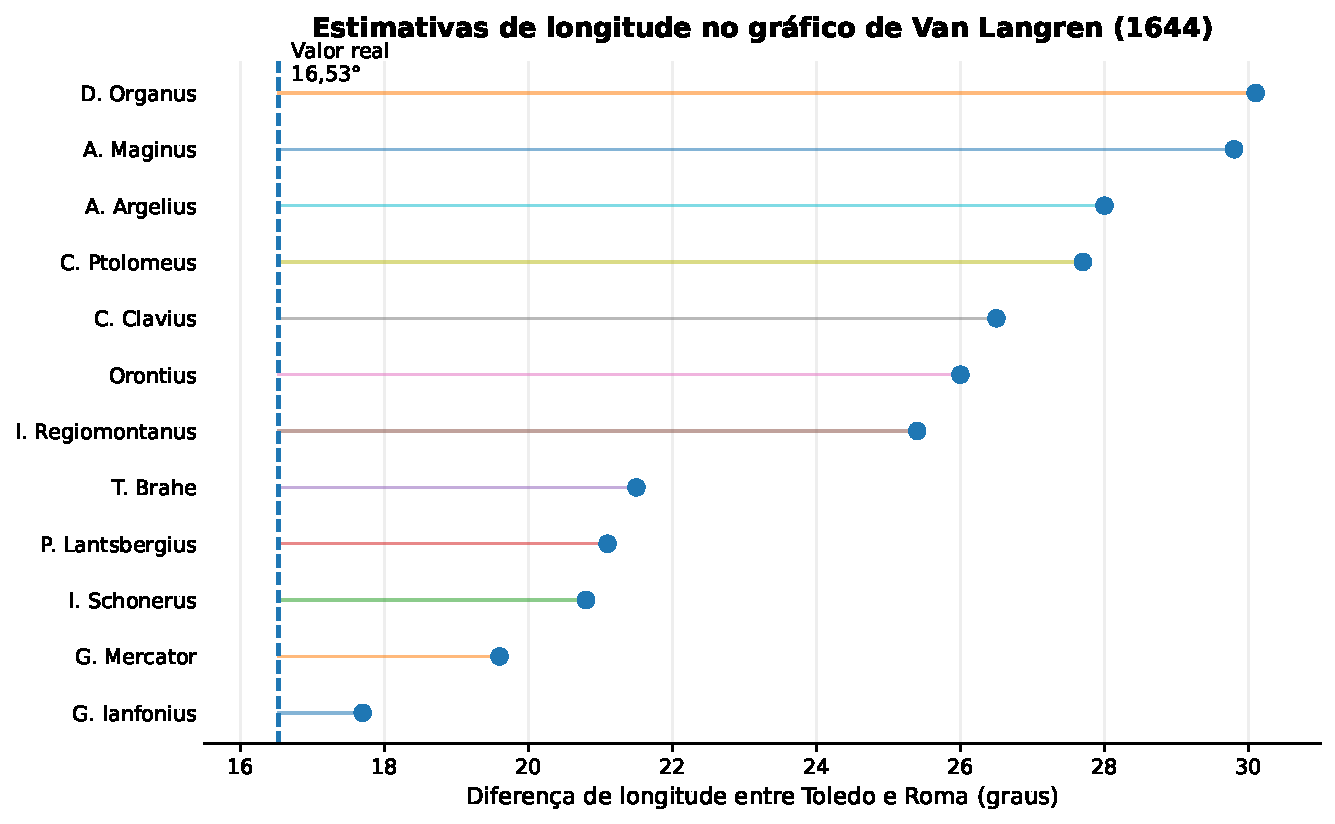
\includegraphics[
                width=\linewidth,
                height=0.52\textheight,
                keepaspectratio
            ]{imagens/van_langren_moderno.pdf}

            \vspace{0.12cm}

            {\scriptsize
            \color{CinzaMedio}
            Dados: \texttt{Langren1644} \parencite{histdata}; \\
            base histórica: \textcite{friendly2010langren}.}

        \end{column}

    \end{columns}

\end{frame}


\begin{frame}{Exemplo 2 — John Snow e a cólera, 1854}

    \vspace{0.05cm}

    \begin{columns}[T,onlytextwidth]


        \begin{column}{0.56\textwidth}

            \etiqueta{MAPA HISTÓRICO}

            \vspace{0.18cm}

            \centering

            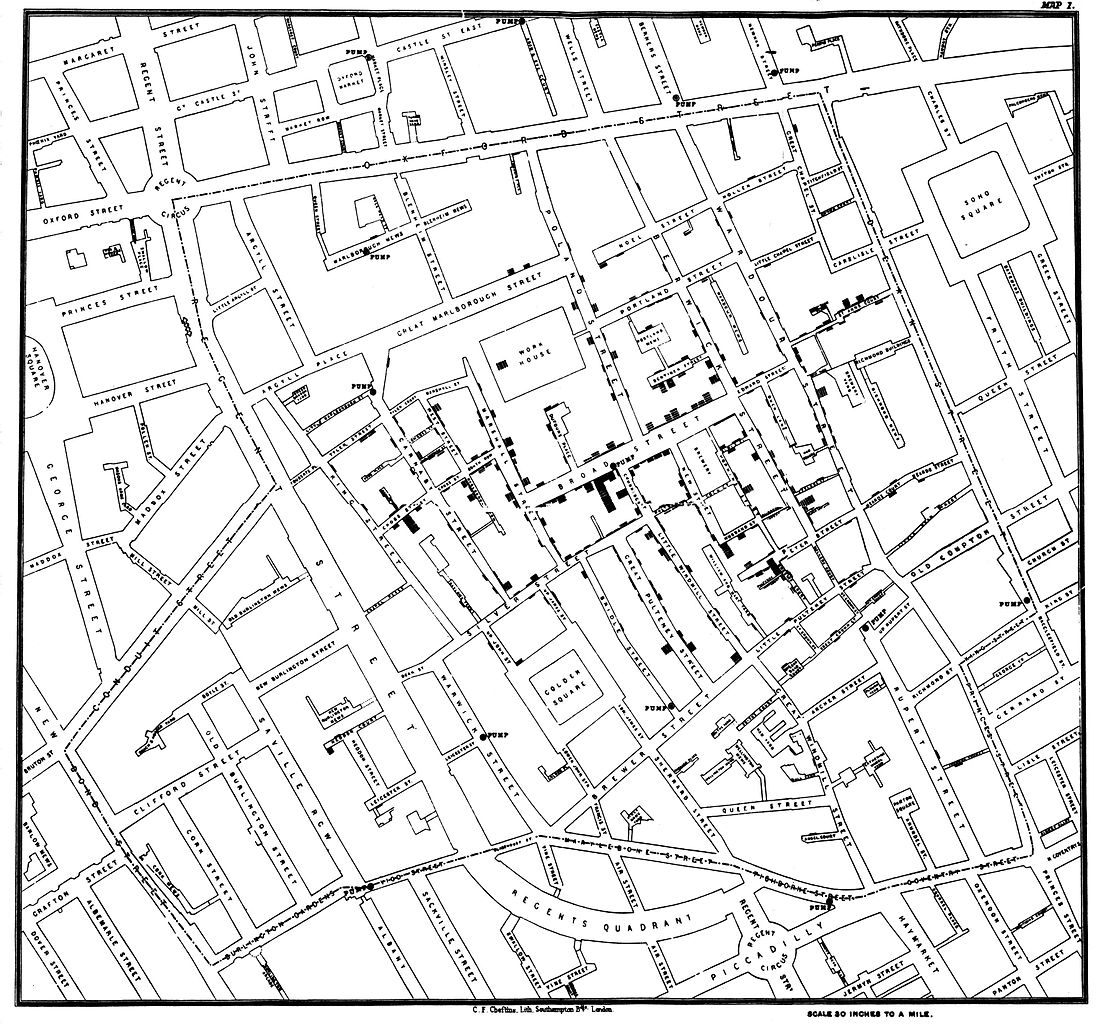
\includegraphics[
                width=0.94\linewidth,
                height=0.58\textheight,
                keepaspectratio
            ]{imagens/john_snow_1854_original.jpg}

            \vspace{0.10cm}

            {\scriptsize
            \color{CinzaMedio}
            Fonte: \textcite{snow1855};
            reproduzido em \textcite{ara2025}.}

        \end{column}


\begin{column}{0.40\textwidth}

    \etiqueta{LEITURA}

    \vspace{0.35cm}

    {\color{AzulEscuro}
    \textbf{O que está sendo mostrado?}}

    \vspace{0.12cm}

    {\small
    A distribuição das mortes por cólera
    no Soho e a localização das bombas
    públicas de água.
    }

    \vspace{0.55cm}

    {\color{AzulEscuro}
    \textbf{O que pode melhorar?}}

    \vspace{0.12cm}

    {\small
    Aumentar o contraste entre os dados
    e o mapa-base e destacar melhor
    as bombas de água.
    }

\end{column}

\end{columns}

\end{frame}


\begin{frame}{O mesmo surto, outra linguagem visual}

    \vspace{0.05cm}

    \begin{columns}[T,onlytextwidth]


        \begin{column}{0.38\textwidth}

            {\color{Sepia}
            \small
            \textbf{O QUE FOI ALTERADO?}}

            \vspace{0.30cm}

            {\color{AzulEscuro}
            \textbf{Contraste}}

            \vspace{0.08cm}

            {\small
            A base do mapa foi escurecida e os casos
            passaram a se destacar visualmente.
            }

            \vspace{0.35cm}

            {\color{AzulEscuro}
            \textbf{Ponto focal}}

            \vspace{0.08cm}

            {\small
            A bomba de Broad Street recebeu maior
            destaque.
            }

            \vspace{0.35cm}

            {\color{AzulEscuro}
            \textbf{Distância}}

            \vspace{0.08cm}

            {\small
            Foram adicionados círculos de distância
            ao redor da bomba para facilitar a leitura
            espacial do surto.
            }

        \end{column}


        \begin{column}{0.58\textwidth}

            {\color{AzulMedio}
            \small
            \textbf{RELEITURA}}

            \vspace{0.15cm}

            \centering

            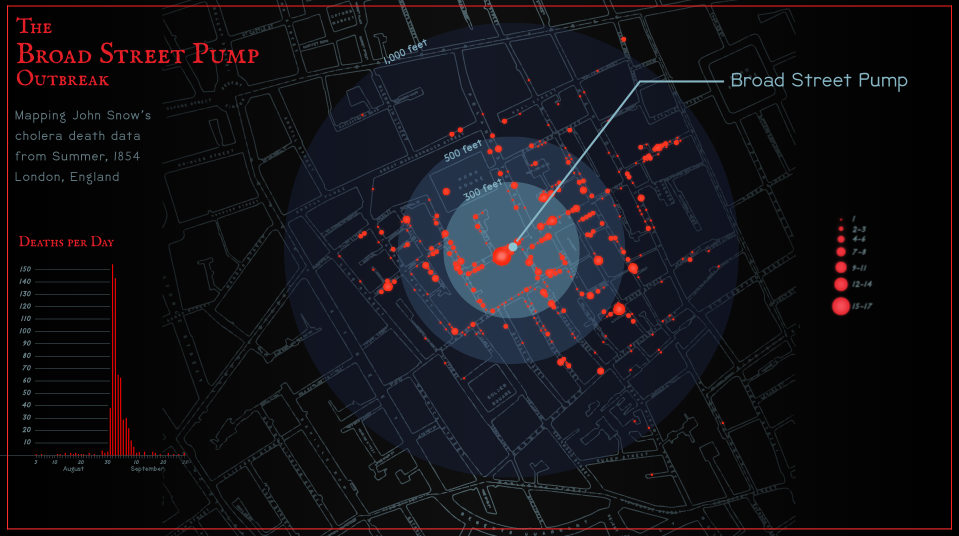
\includegraphics[
                width=0.9\linewidth,
                height=0.61\textheight,
                keepaspectratio
            ]{imagens/john_snow_sarah_bell.png}

            \vspace{0.10cm}

            {\scriptsize
            \color{CinzaMedio}
            Releitura: \textcite{bell2023}. \textit{*Versão animada disponivel na referência.}}

            {\color{AzulEscuro}
            \textbf{Dimensão temporal}}

            \vspace{0.08cm}

            {\small
            Um gráfico de barras foi acrescentado para
            mostrar a evolução das mortes ao longo
            do tempo.
            }

        \end{column}

    \end{columns}

\end{frame}


\begin{frame}{Moderno significa necessariamente melhor?}

    \vfill

    \begin{center}

        {\fontsize{25}{30}\selectfont
        \color{AzulEscuro}
        \textbf{
        Nem toda visualização histórica\\
        precisa ser ``corrigida''.
        }}

        \vspace{0.7cm}

        {\large
        \color{CinzaTexto}

        É importante ressaltar que algumas escolhas feitas há séculos podem continuar
        funcionando porque exploram princípios básicos
        da percepção humana.

        }

    \end{center}

    \vfill

\end{frame}

    
    \begin{frame}{Conclusão}
    
        \begin{columns}[c,onlytextwidth]
    
    
            \begin{column}{0.57\textwidth}
    
        \vspace{0.2cm}
    
        \begin{tikzpicture}
    
            \node[
                draw=AzulMedio,
                rounded corners=5pt,
                minimum height=4.0cm,
                text width=.88\linewidth,
                inner xsep=10pt,
                inner ysep=5pt,
                align=left
            ]{
    
                {\centering
                \large
                \color{AzulEscuro}
                \textbf{Minha conclusão}
                \par}
    
                \vspace{0.15cm}
    
                \small
    
                Mesmo com os recursos disponíveis em sua época,
                os gráficos históricos fazem um ótimo trabalho
                passando a informação que deviam.
    
                \par\vspace{0.25cm}
    
                Reconstruí-los usando princípios modernos
                ajuda a entender como
                contraste, hierarquia, posição e redução
                de ruído alteram a leitura dos dados.
    
                \par\vspace{0.25cm}
    
                Por isso, a reconstrução pode tornar o
                primeiro capítulo muito mais útil
                didaticamente:
    
                \par\vspace{0.12cm}
    
                {\centering
                \textbf{Além de estudar a história,
                ele pode servir como exemplo de como
                construir melhores visualizações.}
                \par}
    
            };
    
        \end{tikzpicture}
    
    \end{column}


        \begin{column}{0.37\textwidth}

            \centering

            \begin{tikzpicture}[
                node distance=0.48cm,
                every node/.style={align=center}
            ]


                \node[
                    draw=Sepia,
                    rounded corners=4pt,
                    line width=1.1pt,
                    text=MarromEscuro,
                    text width=2.7cm,
                    minimum height=0.95cm
                ] (historico) {
                    \small
                    \textbf{Gráfico histórico}
                };


                \node[
                    below=of historico,
                    fill=AzulClaro,
                    rounded corners=4pt,
                    text=AzulEscuro,
                    text width=2.7cm,
                    minimum height=1.15cm
                ] (analise) {
                    \small
                    \textbf{Analisar}\\[-1pt]
                    \scriptsize
                    Gestalt · Tufte\\
                    elementos visuais
                };


                \node[
                    below=of analise,
                    draw=AzulMedio,
                    rounded corners=4pt,
                    line width=1.1pt,
                    text=AzulEscuro,
                    text width=2.7cm,
                    minimum height=0.95cm
                ] (redesenho) {
                    \small
                    \textbf{Redesenhar}
                };


                \node[
                    below=of redesenho,
                    fill=AzulEscuro,
                    rounded corners=4pt,
                    text=Branco,
                    text width=2.7cm,
                    minimum height=1.05cm
                ] (aprendizado) {
                    \small
                    \textbf{Compreender}\\[-1pt]
                    \scriptsize
                    por que o gráfico funciona
                };


                \draw[-{Latex}, thick, Destaque]
                    (historico) -- (analise);

                \draw[-{Latex}, thick, Destaque]
                    (analise) -- (redesenho);

                \draw[-{Latex}, thick, Destaque]
                    (redesenho) -- (aprendizado);

            \end{tikzpicture}

        \end{column}

    \end{columns}

\end{frame}

\begin{frame}[allowframebreaks]{Referências}

    \footnotesize
    \printbibliography

\end{frame}

\end{document}
